% latex - beamer presentation

\documentclass[pdf]{beamer}
\usepackage{beamerthemeshadow}
\mode<presentation>
  {
    \usefonttheme{structuresmallcapsserif}
    \usetheme{PaloAlto}
    %\usecolortheme{seagull}
    %\useinnertheme{circles}
%    \useoutertheme{tree}
  }

\usepackage{xmpmulti}

\usepackage{hyperref}
\hypersetup{
    pdffitwindow=true,     % window fit to page when opened
    colorlinks=true,       % false: boxed links; true: colored links
    linkcolor=orange,          % color of internal links (change box color with linkbordercolor)
    citecolor=green,        % color of links to bibliography
    filecolor=magenta,      % color of file links
    urlcolor=blue           % color of external links
}


\graphicspath{{Figures/}}

\begin{document}
\title{Periodic Motion}  
\author{Caltech: ph2a}
\date{26 - Sep - 2017}
%\logo{
\includegraphics[height=0.5cm]{../caltech_logo.png}}

\frame{\titlepage} 

\frame{\frametitle{Table of contents}\tableofcontents} 


\section{Class Overview}
\frame{\frametitle{Overview}
\begin{enumerate}
\item All info on class website: \url{https://piazza.com/caltech/fall2017/ph2a}
\item Lectures are Tuesday and Thursday
\item try out different sections; problems solving is key!
\item Use piazza for group chat / anon discussions, feedback
\item HWK due every Wed. Quizzes every other Tuesday. Final in Dec.

\end{enumerate}
}


\section{Simple Harmonic Oscillator}
\frame{\frametitle{The Simple Harmonic Oscillator}
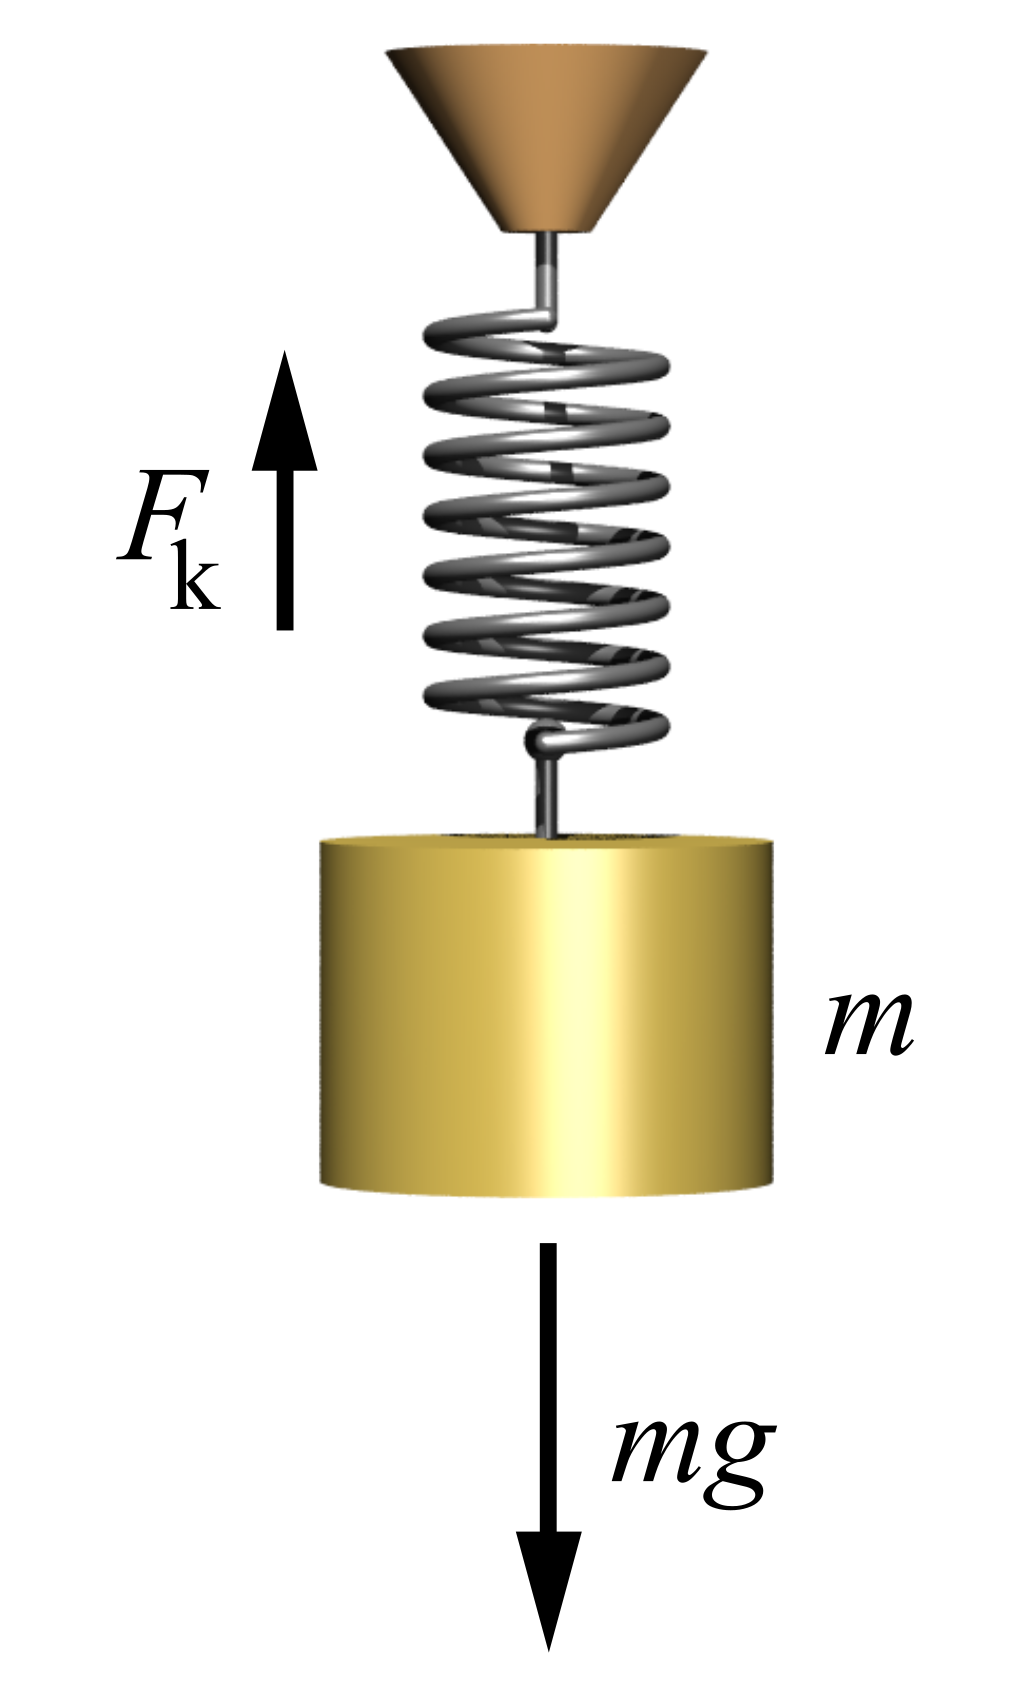
\includegraphics[height=3cm]{Mass-spring-system.png}

\begin{itemize}
\item Covered in ph1a (mass-spring, pendulums) \pause
\item Covered in ph1b/c (RLC Circuits) \pause
\item Extremely useful in engineering / sciences \pause
\item ``Just'' the study of 2$^{nd}$ order differential equations
\end{itemize}

}

\subsection{Demo: Ball on Spring}
\frame{\frametitle{Interactive Demo}
\centering
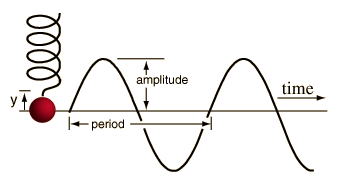
\includegraphics[height=3cm]{2015416-94550395-2754-sshm.png}

}
\subsection{General Solution}
\frame{\frametitle{Harmonic Oscillator Equations}
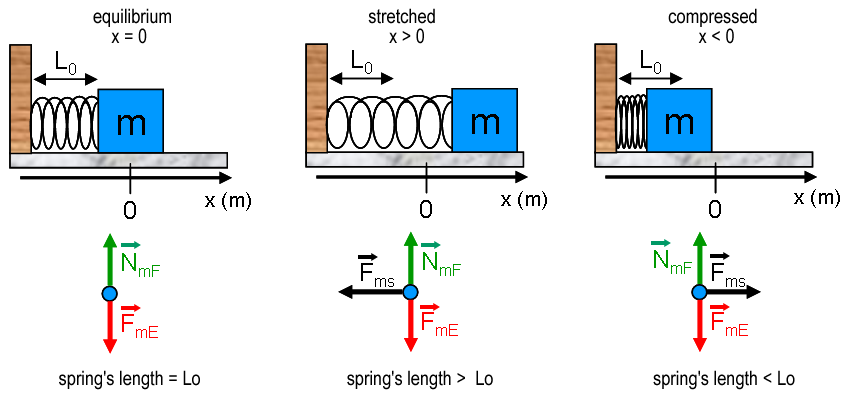
\includegraphics[height = 2cm]{Hookeslawb.png} \\ \pause
$F = m a$ \\ \pause
$- k x = m \frac{d^2x}{dt^2} $
}

\frame{\frametitle{Solution I:}
\begin{align}
  \onslide<1->{x(t) &= A cos(\omega t) + B sin(\omega t) \\}
  \onslide<2->{\frac{dx}{dt} &= -\omega A sin(\omega t) + \omega B cos(\omega t) \\}
  \onslide<3->{\frac{d^2x}{dt^2} &= -\omega^2 \left[A cos(\omega t) + B sin(\omega t)\right] \\}
                 \onslide<4->{&= -\omega^2 x(t)}
\end{align}
\pause
Therefore, $\omega = \sqrt{k/m}$.
}

\frame{\frametitle{Solution II:}
\begin{align}
  \onslide<1->{x(t) &= D cos(\omega t + \phi_0) \\}
  \onslide<2->{\frac{dx}{dt} &= -\omega D sin(\omega t + \phi_0) \\}
  \onslide<3->{\frac{d^2x}{dt^2} &= -\omega^2 D cos(\omega t + \phi_0) \\}
                 \onslide<4->{&= -\omega^2 x(t)}
\end{align}
}

\frame{\frametitle{Boundary Conditions}
In both cases, there are two free constants (A \& B, or D \& $\phi_0$). \\

These constants are set to force the solution to match any 'Boundary' conditions:
\begin{itemize}
\item initial displacement \pause
\item initial velocity \pause
\item e.g., mass is released at t=0 with x = x$_0$
\end{itemize}

}

\subsection{Damping / Friction}
%\begin{frame}
%  \transduration<0-47>{0}
%  \multiinclude[<+->][format=png, graphics={height=2cm}]{AnimMassSpring/Animated-mass-spring}
%\end{frame}


\section{Differential Equations} 
\subsection{Tables}
\frame{\frametitle{Tables}
\begin{tabular}{|c|c|c|}
\hline
\textbf{Date} & \textbf{Instructor} & \textbf{Title} \\
\hline
WS 04/05 & Sascha Frank & First steps with  \LaTeX  \\
\hline
SS 05 & Sascha Frank & \LaTeX \ Course serial \\
\hline
\end{tabular}}


\frame{\frametitle{Tables with pause}
\begin{tabular}{c c c}
A & B & C \\ 
\pause 
1 & 2 & 3 \\  
\pause 
A & B & C \\ 
\end{tabular} }


\section{Harmonic Oscillator + Complex Math}
\subsection{blocs}
\frame{\frametitle{blocs}

\begin{block}{title of the bloc}
bloc text
\end{block}

\begin{exampleblock}{title of the bloc}
bloc text
\end{exampleblock}


\begin{alertblock}{title of the bloc}
bloc text
\end{alertblock}
}


\section{Damped Harmonic Oscillator}


\end{document}

